\chapter{Overview of Our Approach}
\label{chap.ourapproach}

The sample \figref{fig.float} shows ...

\begin{figure}[htb]
\begin{center}
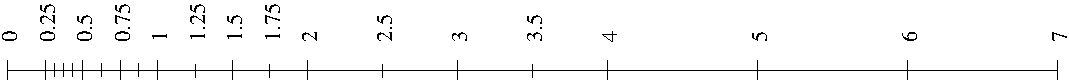
\includegraphics[width=.95\textwidth]{pic/float.pdf}
\end{center}
\caption{Distribution of the floating point numbers. This figure shows a distribution of a sample floating point number set with a precision $t=3$, and $e_{min}=-1$ and $e_{max}=3$.}
\label{fig.float}
\end{figure}


There are two basic floating point \index{Floating point} data types \index{Floating point!Data types}, as defined by the IEEE 754-2008 \cite{ieee754} standard, are shown in \tabref{tab.floatingpointdatatypes}.

\begin{table}[htb]
\begin{center}
\begin{tabular}{|r|c|c|c||c||c|}
% Draw horizontal table line from column 2 to column 6
% The first column is left empty, without the horizontal line
\cline{2-6}

% Since we do not want to change the formatting of the first column
% we need to use the multicolumn macro \multicolumn{#ofcolumns}{newformatting}{content}
% so we can change |r| to just r|. If we did not do that, we'd have the left
% vertical line drawn in the first column. Also in order to make the header row
% nicer, we use the \vrule macro. See below for an explanation.
\multicolumn{1}{r|}{} & {\vrule height 13pt depth 6pt width 0pt\bf Sign} [b] & {\bf Exponent} [b] & {\bf Mantissa} [b] & {\bf Prec.} [dig] & {\bf Total} [b]\\ \cline{2-6}  \hline

% This vrule shows that we can extend the column height or depth if necessary.
% This is useful for header rows or rows that contain some mathematical expressions.
\vrule height 10pt depth 20pt width 0pt
{\bf binary32}   			& 1    & 8        	& 24      & 8  	& 32\\ \hline

% To debug, make the vertical rule visible by specifying its width to 1 pt rather than 0 pt.
\vrule height 20pt depth 0pt width 1pt
{\bf binary64}   			& 1    & 11       	& 53      & 16	& 64\\ \hline
\end{tabular}
\end{center}
\caption{Basic floating point data types.}
\label{tab.floatingpointdatatypes}
\end{table}
